\documentclass{beamer}

\usepackage{beamerthemesplit} 
\usetheme{Warsaw}
\usecolortheme{beetle}
\setbeamercolor{background canvas}{bg = white}

\title{\color{gray}Cellular Automata}
\author{Joy Kimmel}
\date{May 7, 2014}
\institute{Gordon College}


\begin{document}


\frame{\titlepage}

\section{Outline}

\frame
{
\frametitle{Overview}
\begin{itemize}
	\item<1-> Introduction
	\item<2-> "Game Of Life"
		\begin{itemize}
		\item Rules
		\item Code
		\item Results
		\end{itemize}
	\item<3-> Sandpile Model
		\begin{itemize}
		\item Algorithm / Code
		\item Results
		\item Properties
		\end{itemize}
	\item<4-> Conclusion
\end{itemize}
 }
 
\section{Introduction}
\subsection{Background}
\frame
{
  \frametitle{What is Cellular Automata?}

  \begin{itemize}
  	\item Approach to modeling the time evolution of a system
  	\item Usually deterministic rules
	\item Many applications
  \end{itemize}
 
  \begin{definition}
  \textit{cellular}: "discrete space and local nature" \\
  \textit{automata}: "rule-based automatic time evolution"
  \end{definition}
}


\subsection{Basic Principles}
\frame
{
  \frametitle{General Steps}
  \begin{itemize}
  	\item Choose cellular space (LxL lattice)
  	\begin{figure}
	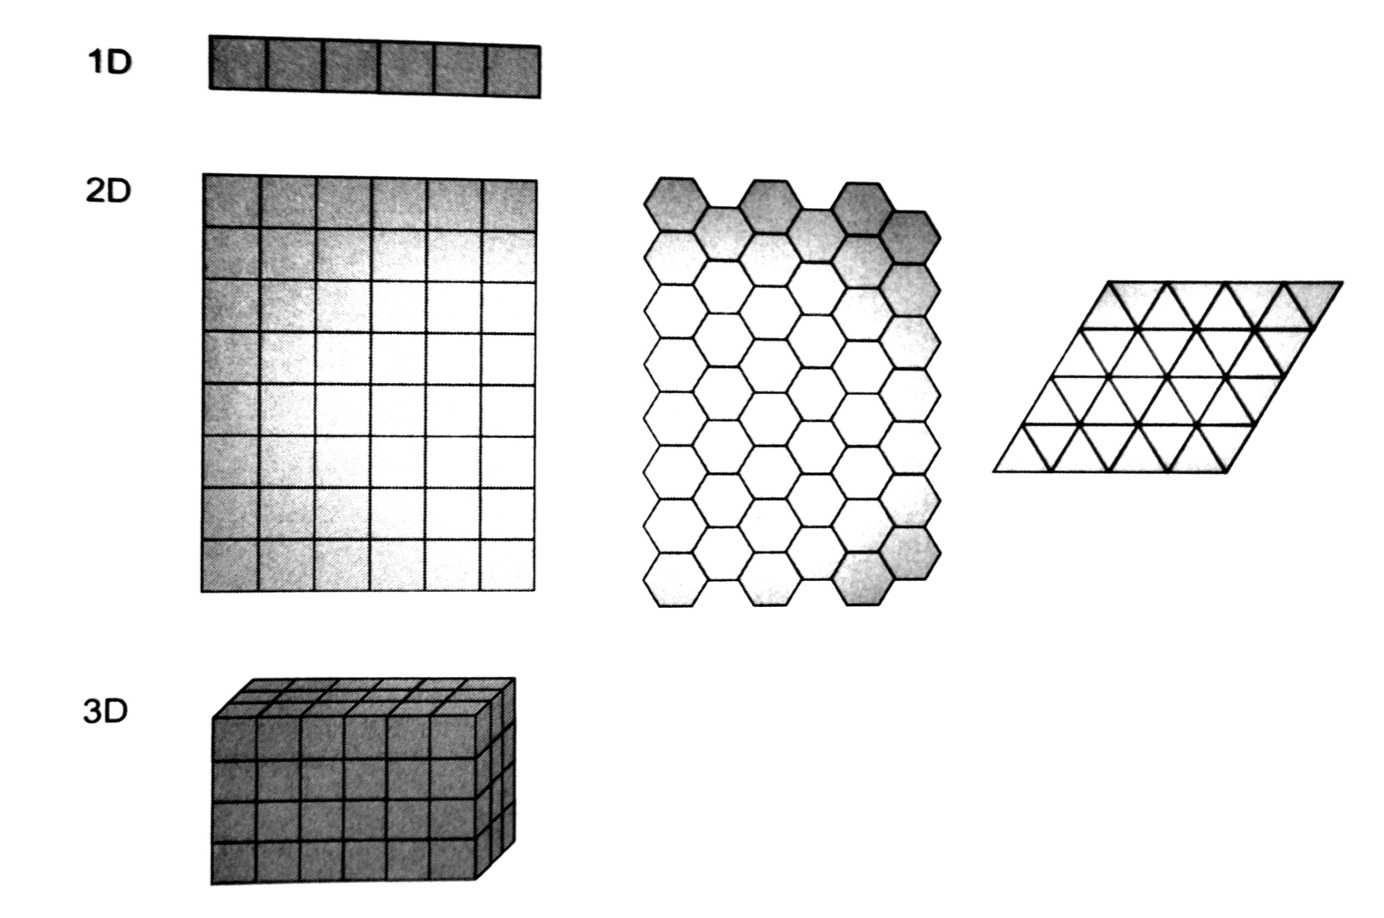
\includegraphics[width = 200, align=right]{lattice}
	\end{figure}
  \end{itemize}
}



\frame
{
\begin{itemize}
  \item<1-> Assign the state set:  S
      	\begin{itemize}
	\item For the simplest example: a block can either be 'occupied' or 'unoccupied'
	\end{itemize}
  \item<2-> Choose neighbors
    	\begin{itemize}
		\item von Neumann
		\item Moore
	\end{itemize}
	
	\begin{figure}
	\includegraphics<2->[width = 200, align=right]{neighborhood}
	\end{figure}
    \end{itemize}
}


\frame
{
 \begin{itemize}
  \item<1-> Choose transition rules 
  	\begin{itemize}
	\item Number of possible transition rules (TR) grows with possible states (k) and number of neighbors (n)
	\item Follows the equation: ${k^{k}}^{n}$
	\item With k $= 2$ possible states, n $= 3$ neighbors:  TR $= {2^{2}}^{3} = 256$ 
	\item With k $= 3$ possible states, n $= 3$ neighbors: \\ TR $= {3^{3}}^{3} = 7,625,597,484,987$	
	\end{itemize}
  \item<2-> Choose a time variable: continuous or discrete
  \item<3-> Assign boundary conditions
  \item<4-> Assign initial conditions
  \item<5-> Assign a stopping condition
  \item<6-> Repeat until the stopping condition is met
  \end{itemize}
}


\subsection{Applications}
\frame
{
  \frametitle{Concrete Examples}

  \begin{itemize}
  \item "Game Of Life"
  \item Forest Fires
  \item Maze Solution 
  \item Traffic Simulation
  \item Social Dynamics
  \end{itemize}

}

\frame
{
  \frametitle{Traffic Simulation}

  	\begin{figure}
	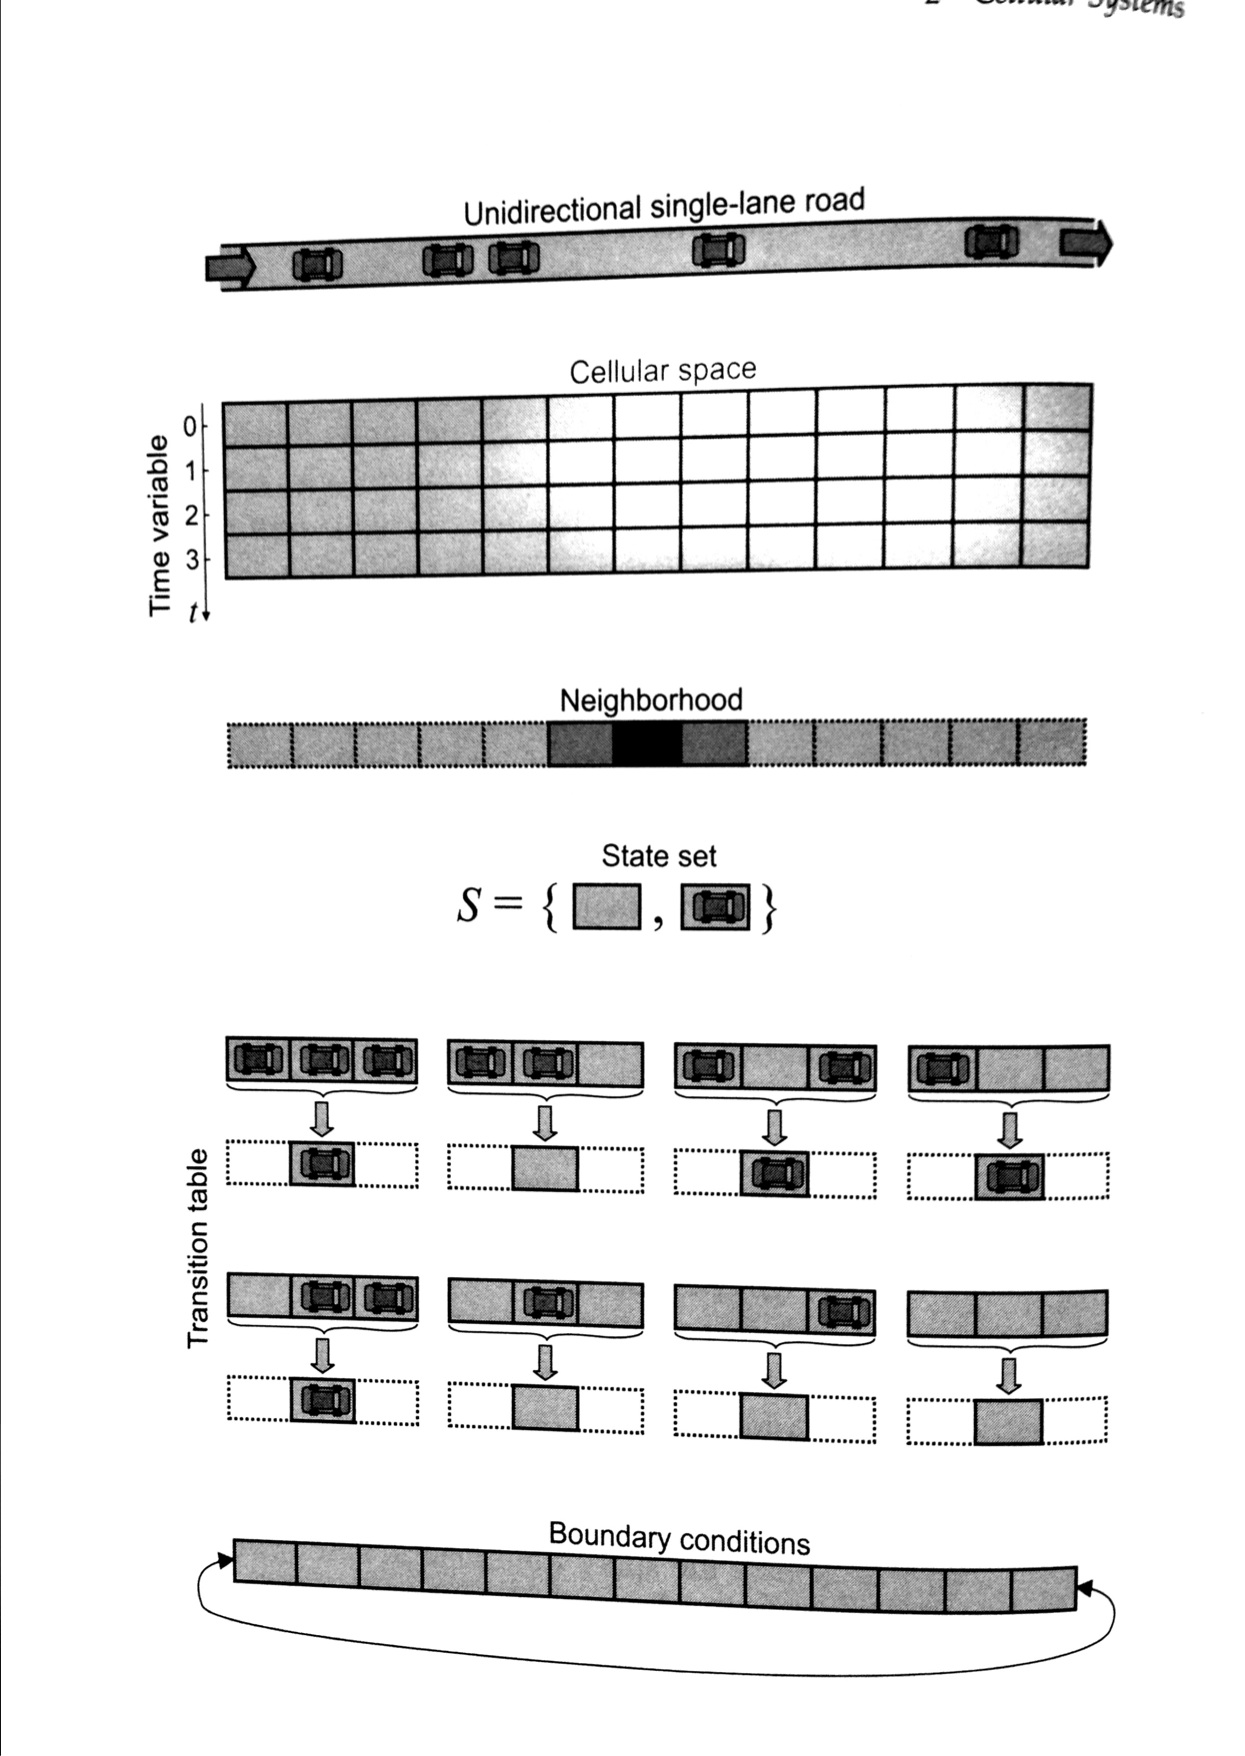
\includegraphics[height = 130, align=right]{traffic}
	\end{figure}

}

\frame
{
  \frametitle{Social Dynamics}

  \begin{figure}
	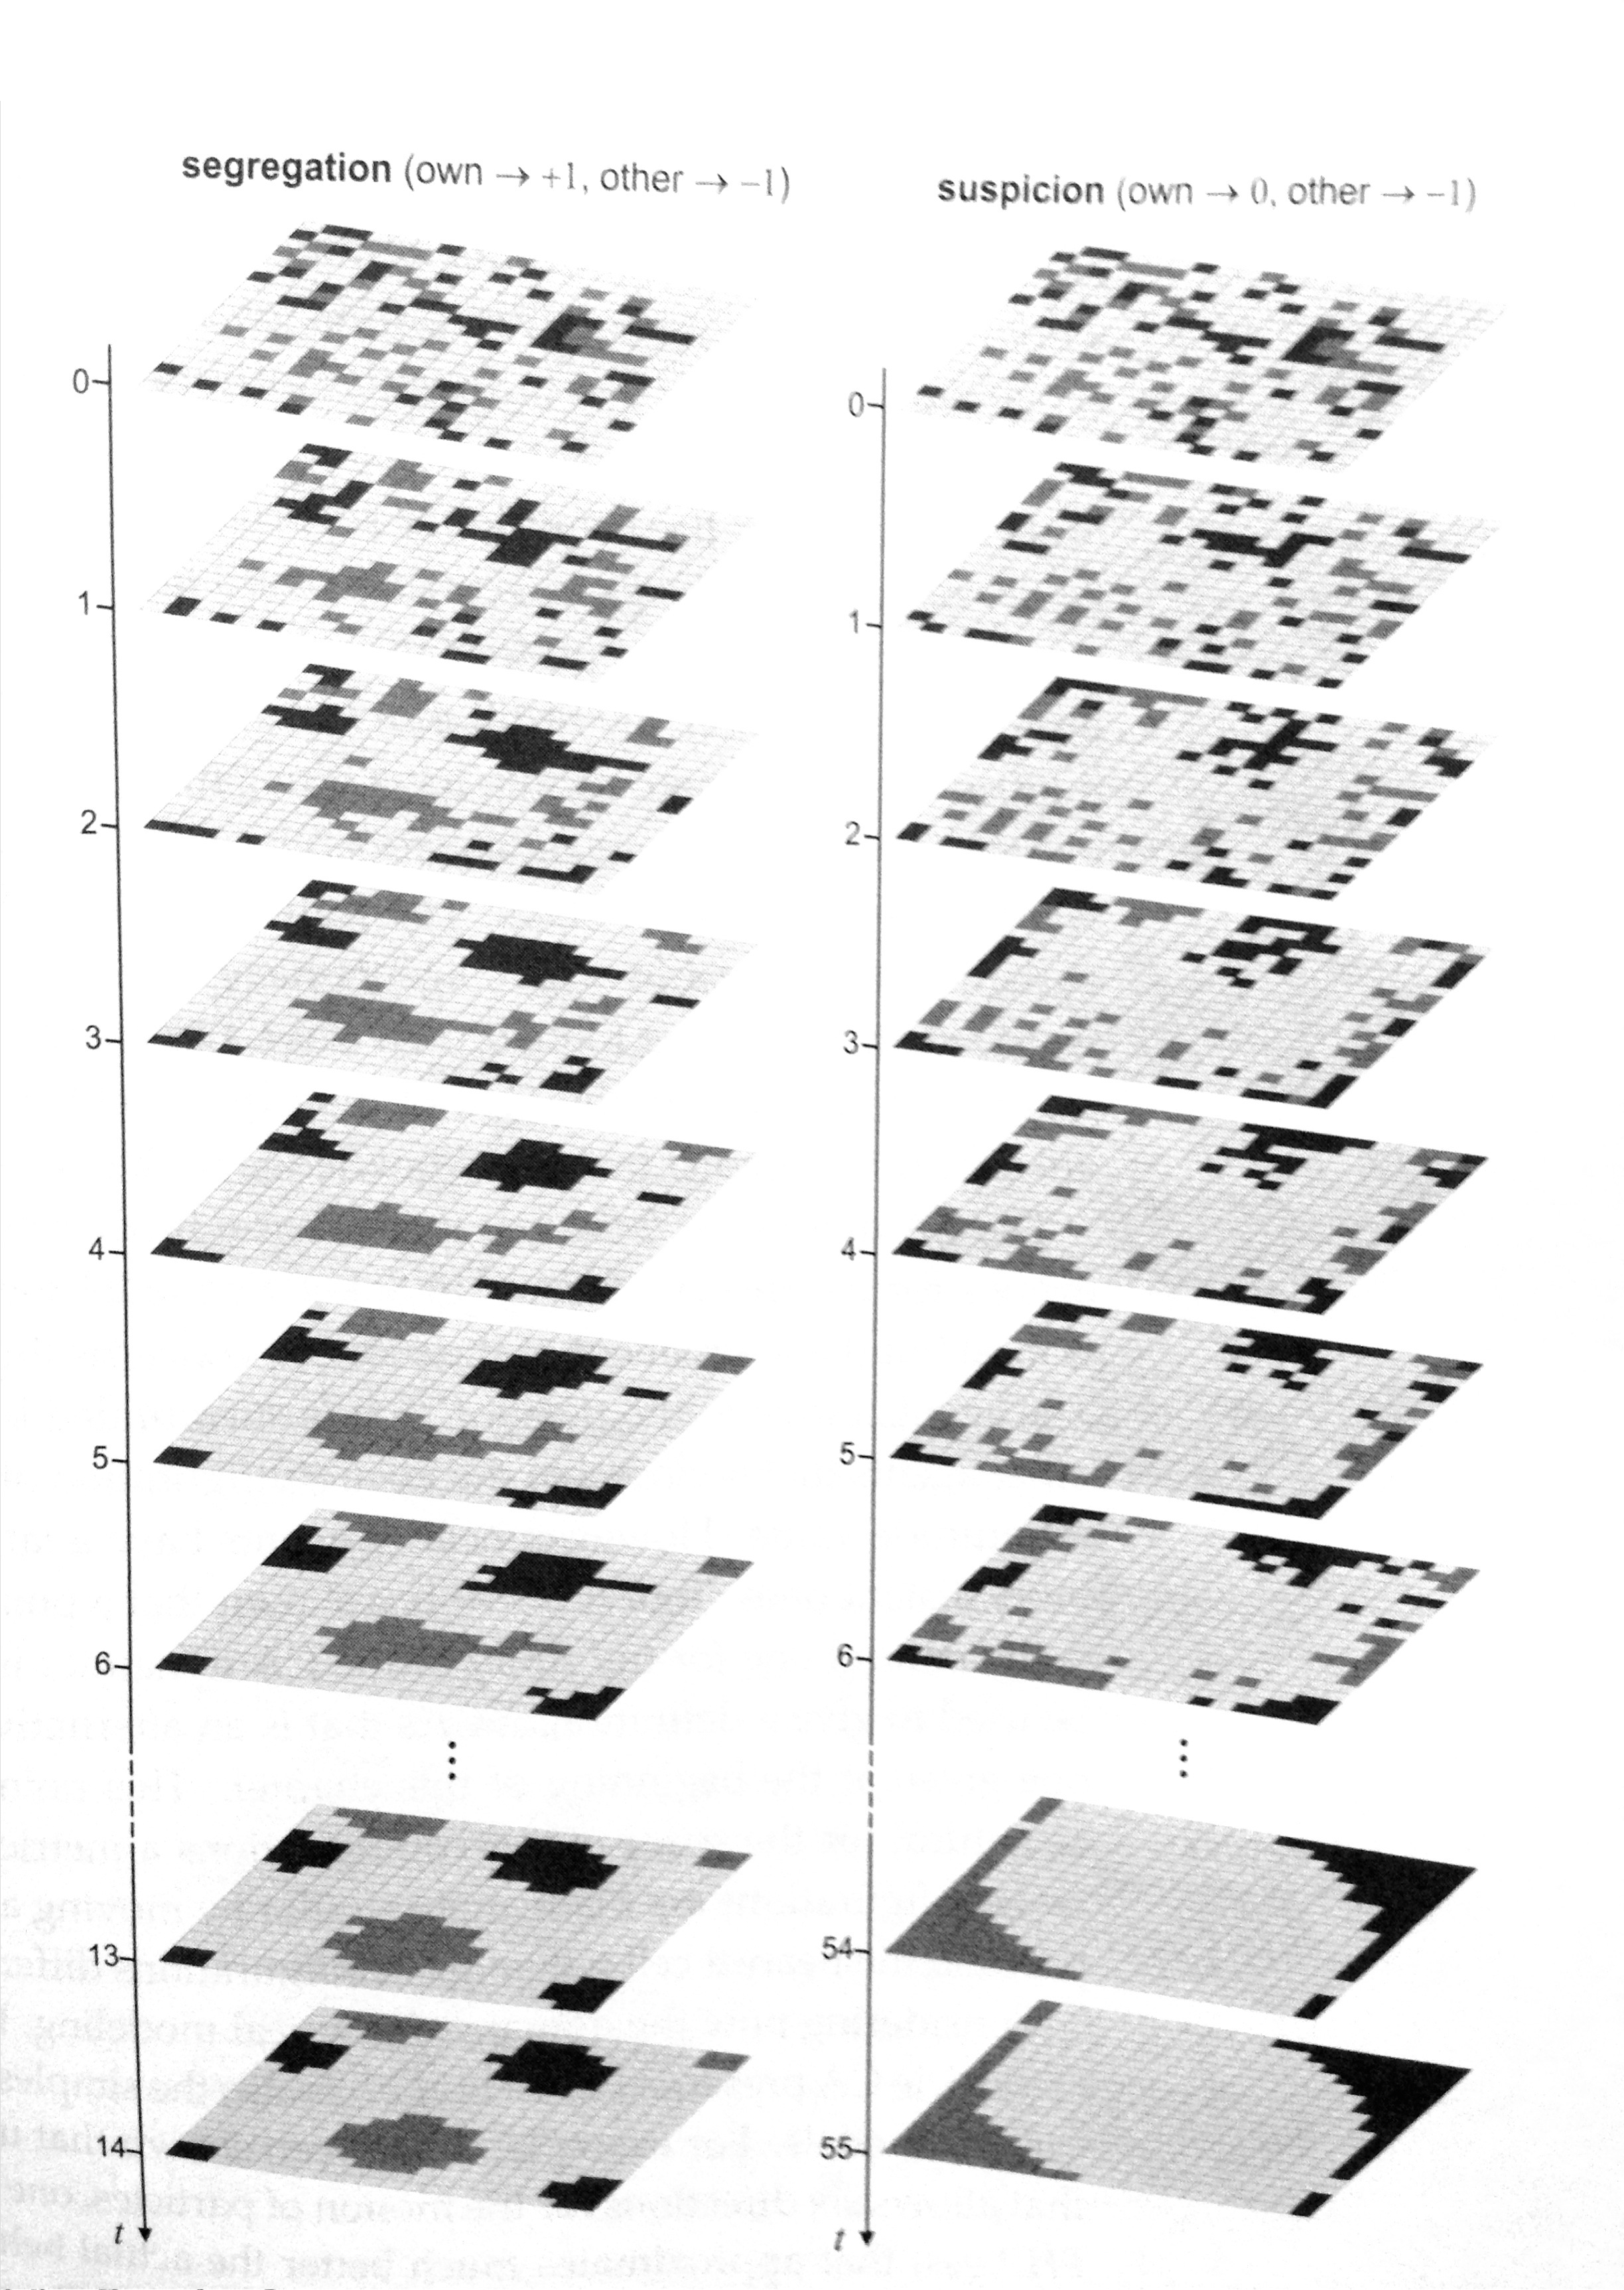
\includegraphics[width = 120, align=right]{social}
\end{figure}
  

}

\section{"Game Of Life"}
\subsection{Introduction}
\frame
{
  \frametitle{Background / History}

  \begin{itemize}
  \item Introduced by Conway in 1970
  \item 8 neighbors (Moore)
  \item A cell is either "alive" or "dead"
  \item Discrete time steps
  \end{itemize}
}

\subsection{Rules}
\frame
{
  \frametitle{Simple Algorithm}

  \begin{itemize}
  \item<1-> If 2 neighbors are alive: the state of the cell in the next time step is unchanged
  \item<2-> If 3 neighbors are alive: the state of the cell is alive no matter its current state 
  \item<3-> Otherwise the cell is dead
  \end{itemize}  
}


\subsection{Results}
\frame
{
  \frametitle{Simple Patterns: Blinker}
  \begin{figure}
   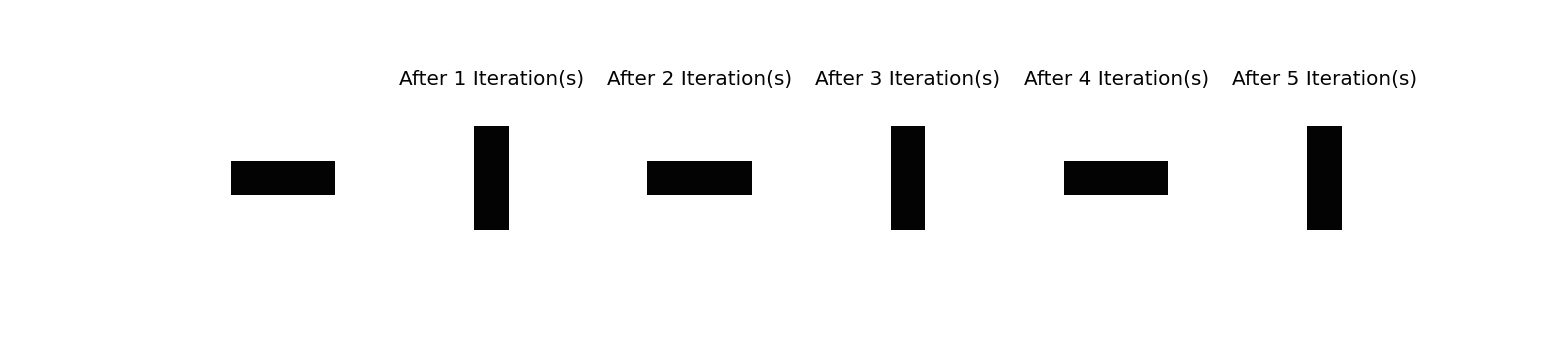
\includegraphics[width = 300]{simpleblinker}
   \end{figure}
}
\frame
{
  \frametitle{Simple Patterns: Glider}
  \begin{figure}
   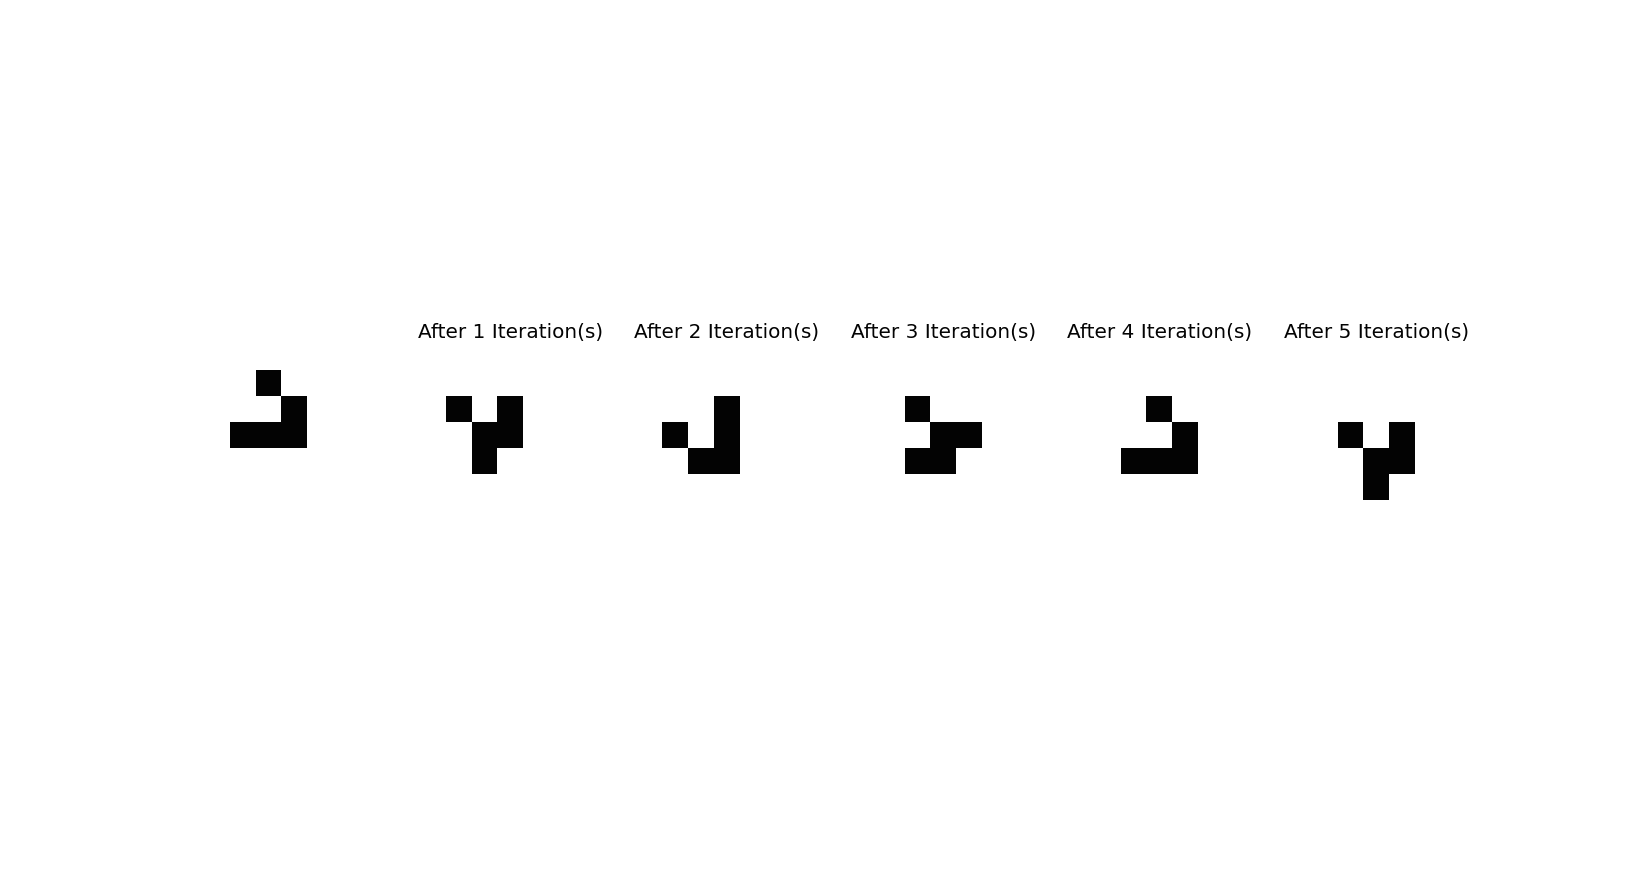
\includegraphics[width = 300]{simpleglider}
   \end{figure}

}

\frame
{
  \frametitle{Chaotic Behavior}

 \begin{itemize}
  \item 100x100 Lattice
  \item Randomly generated an initial condition [with a probability of being alive: $0.3$]
  \item White: never alive, Gray: once alive - now dead, Black: dead
  \item See code (via handout)
  \end{itemize}
  
}

\frame
{
  \frametitle{Chaotic Behavior}
    \begin{figure}
   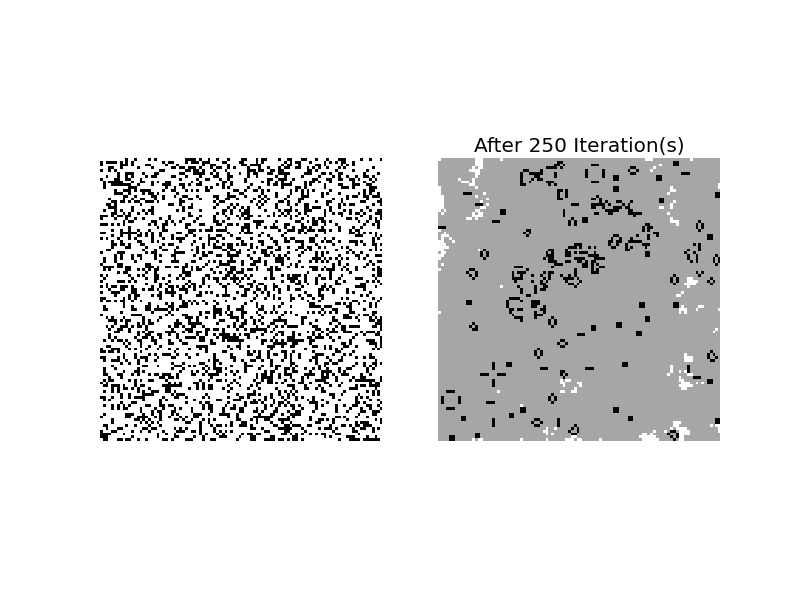
\includegraphics[width = 300]{chaotic}
   \end{figure}
}



\subsection{Change of Rules}
\frame
{
  \frametitle{Simple Algorithm - Generalized}

  \begin{itemize}
  \item If n neighbors are alive: the state of the cell in the next time step is unchanged
  \item If n+1 neighbors are alive: the state of the cell is alive no matter its current state 
  \item Otherwise the cell is dead
  \end{itemize}  
}


\subsection{Results}
\frame
{
  \frametitle{"Blinker" at n = 1}
  \begin{figure}
   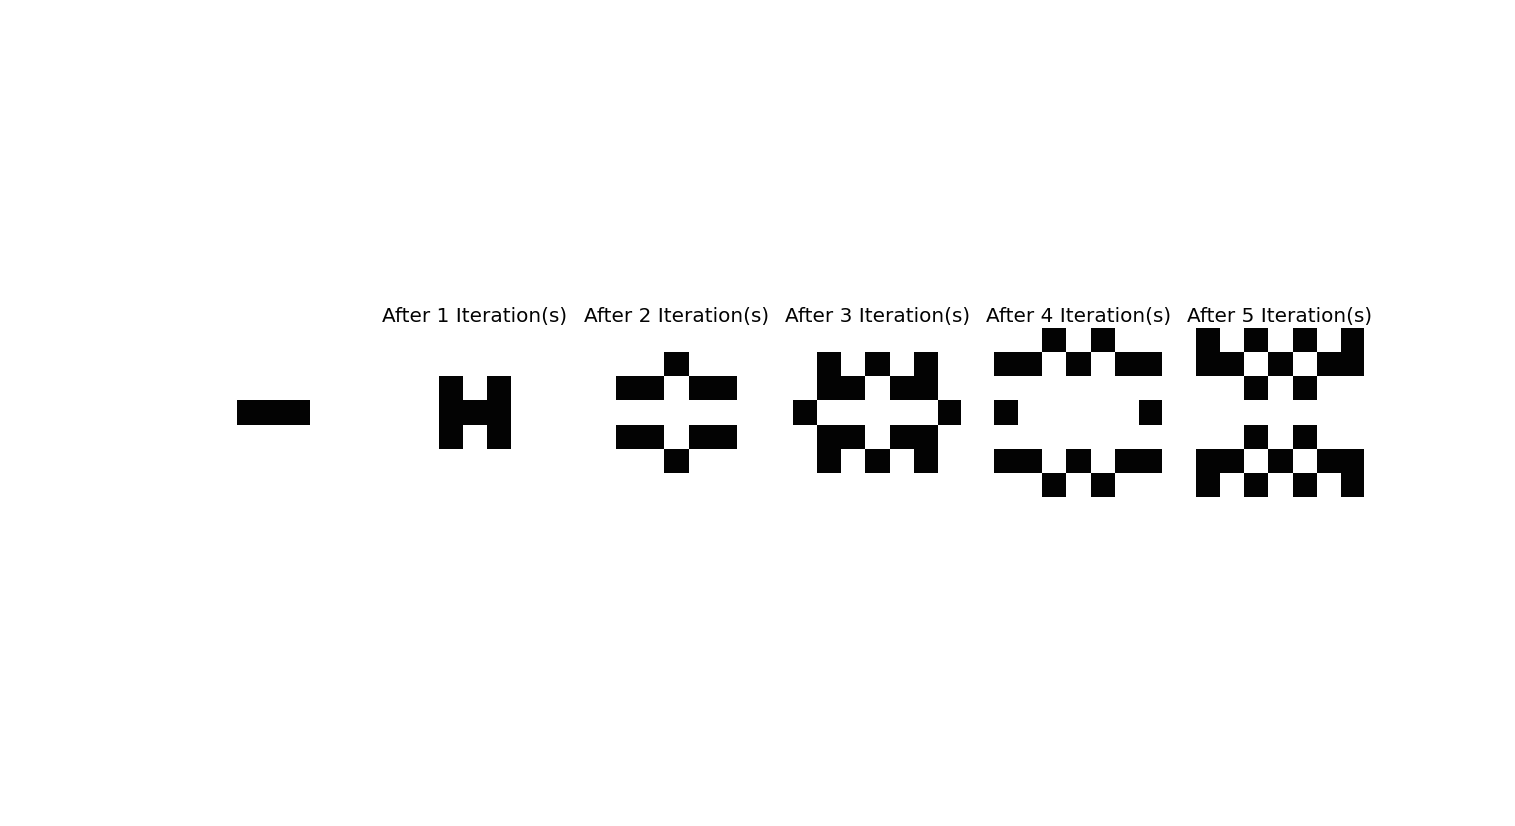
\includegraphics[width = 300]{blinker12}
   \end{figure}
}

\frame
{
 \frametitle{"Glider" at n = 1}
  \begin{figure}
   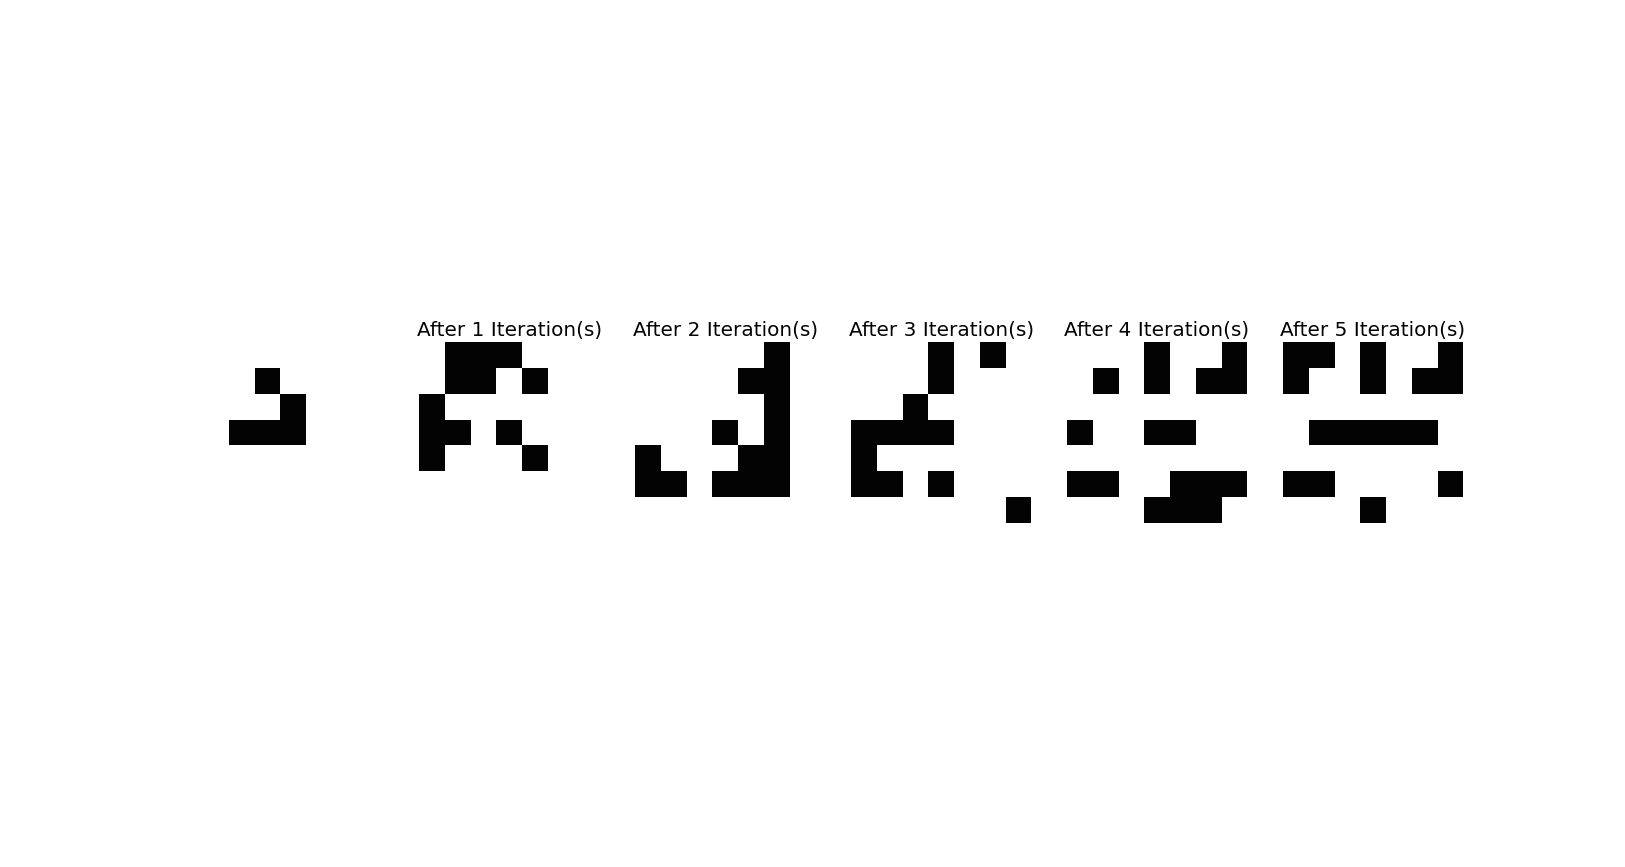
\includegraphics[width = 300]{glider12}
   \end{figure}

}


\frame
{
  \frametitle{Chaotic Behavior}

 \begin{itemize}
  \item 100x100 Lattice
  \item Randomly generated an initial condition [with a probability of being alive: $0.1$]
  \item White: never alive, Gray: once alive - now dead, Black: dead
  \end{itemize}  
  
}

\frame
{
  \frametitle{Chaotic Behavior}
   \begin{figure}
   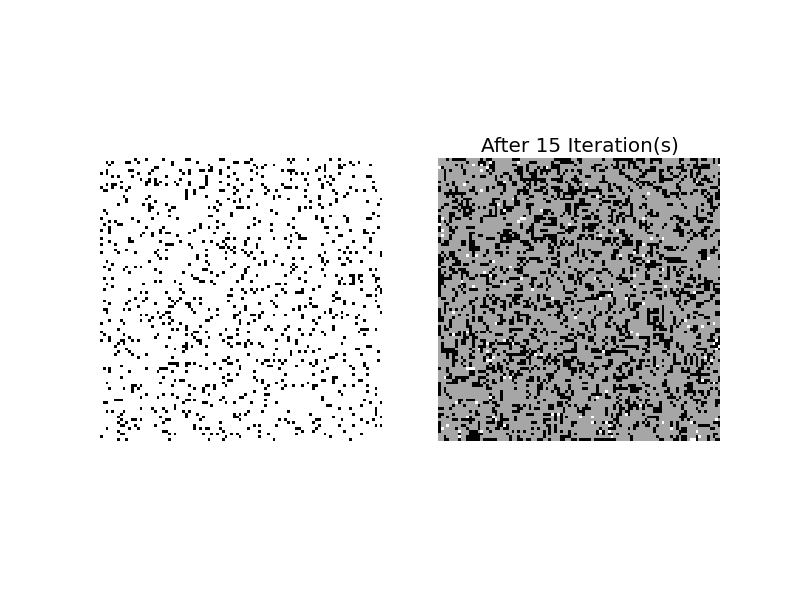
\includegraphics[width = 300]{chaos12}
   \end{figure}

}

\frame
{
\frametitle{Additional Rules and Results}
\begin{figure}
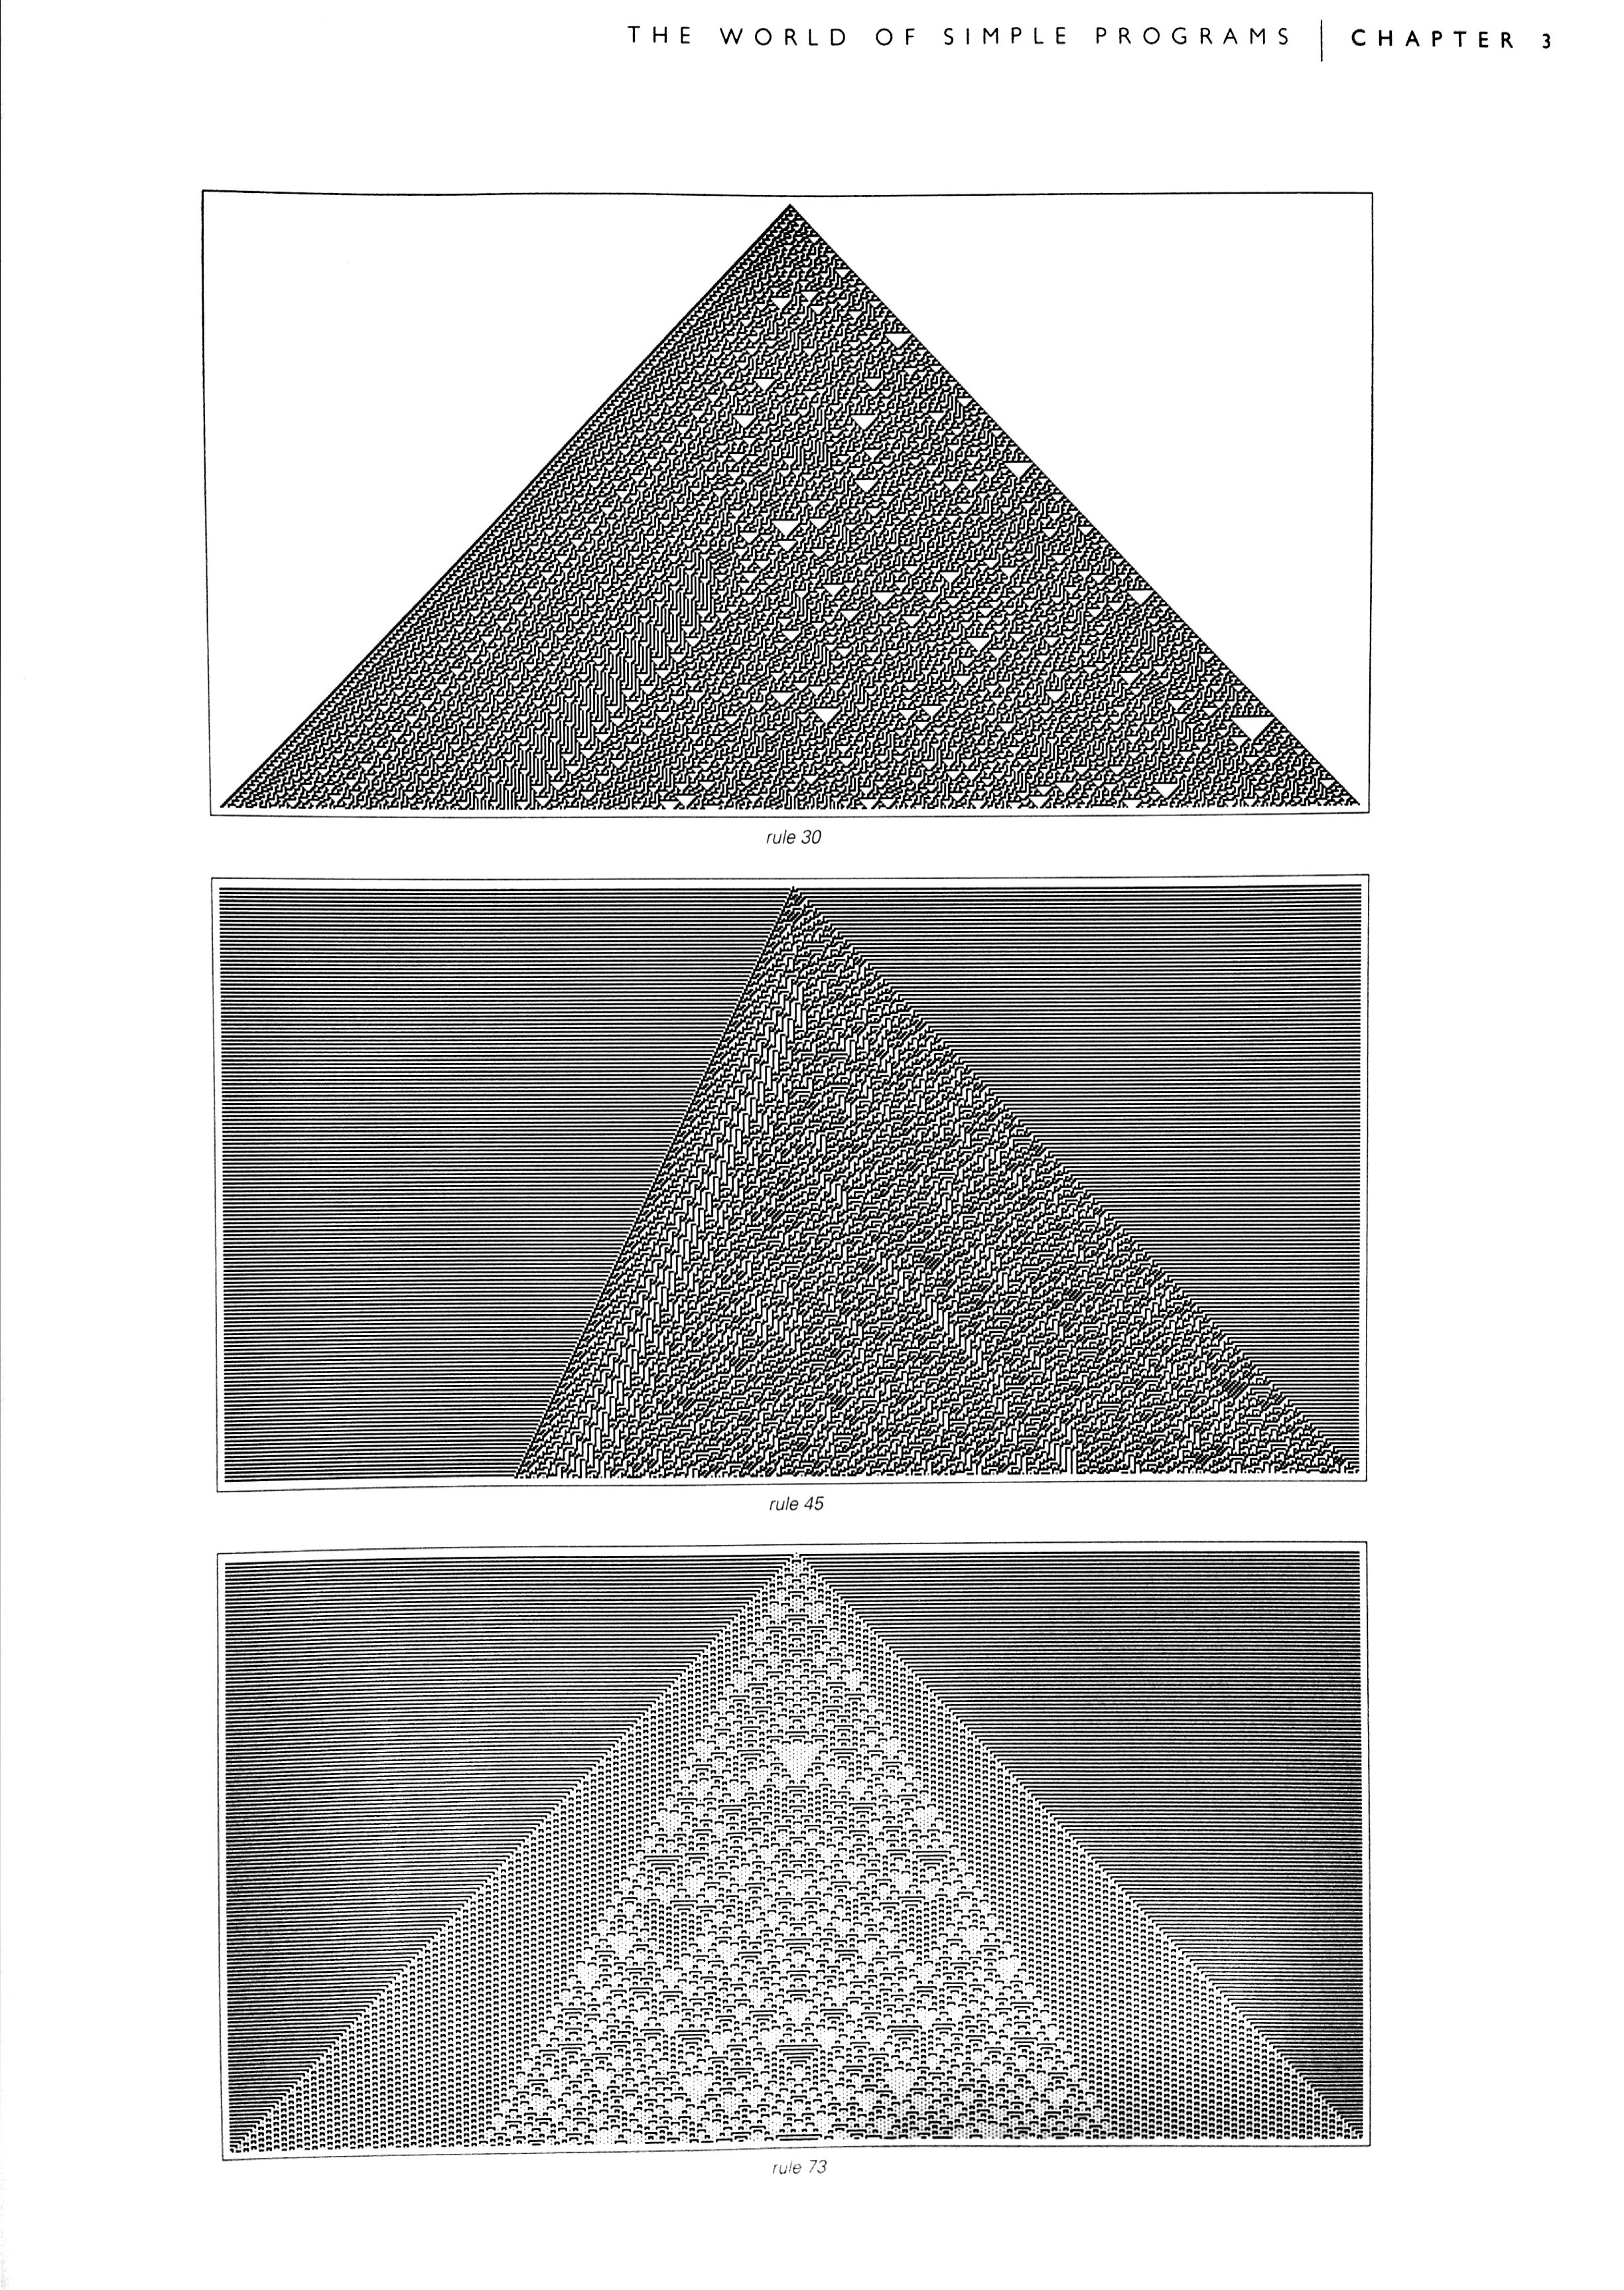
\includegraphics[width = 100]{triangle}
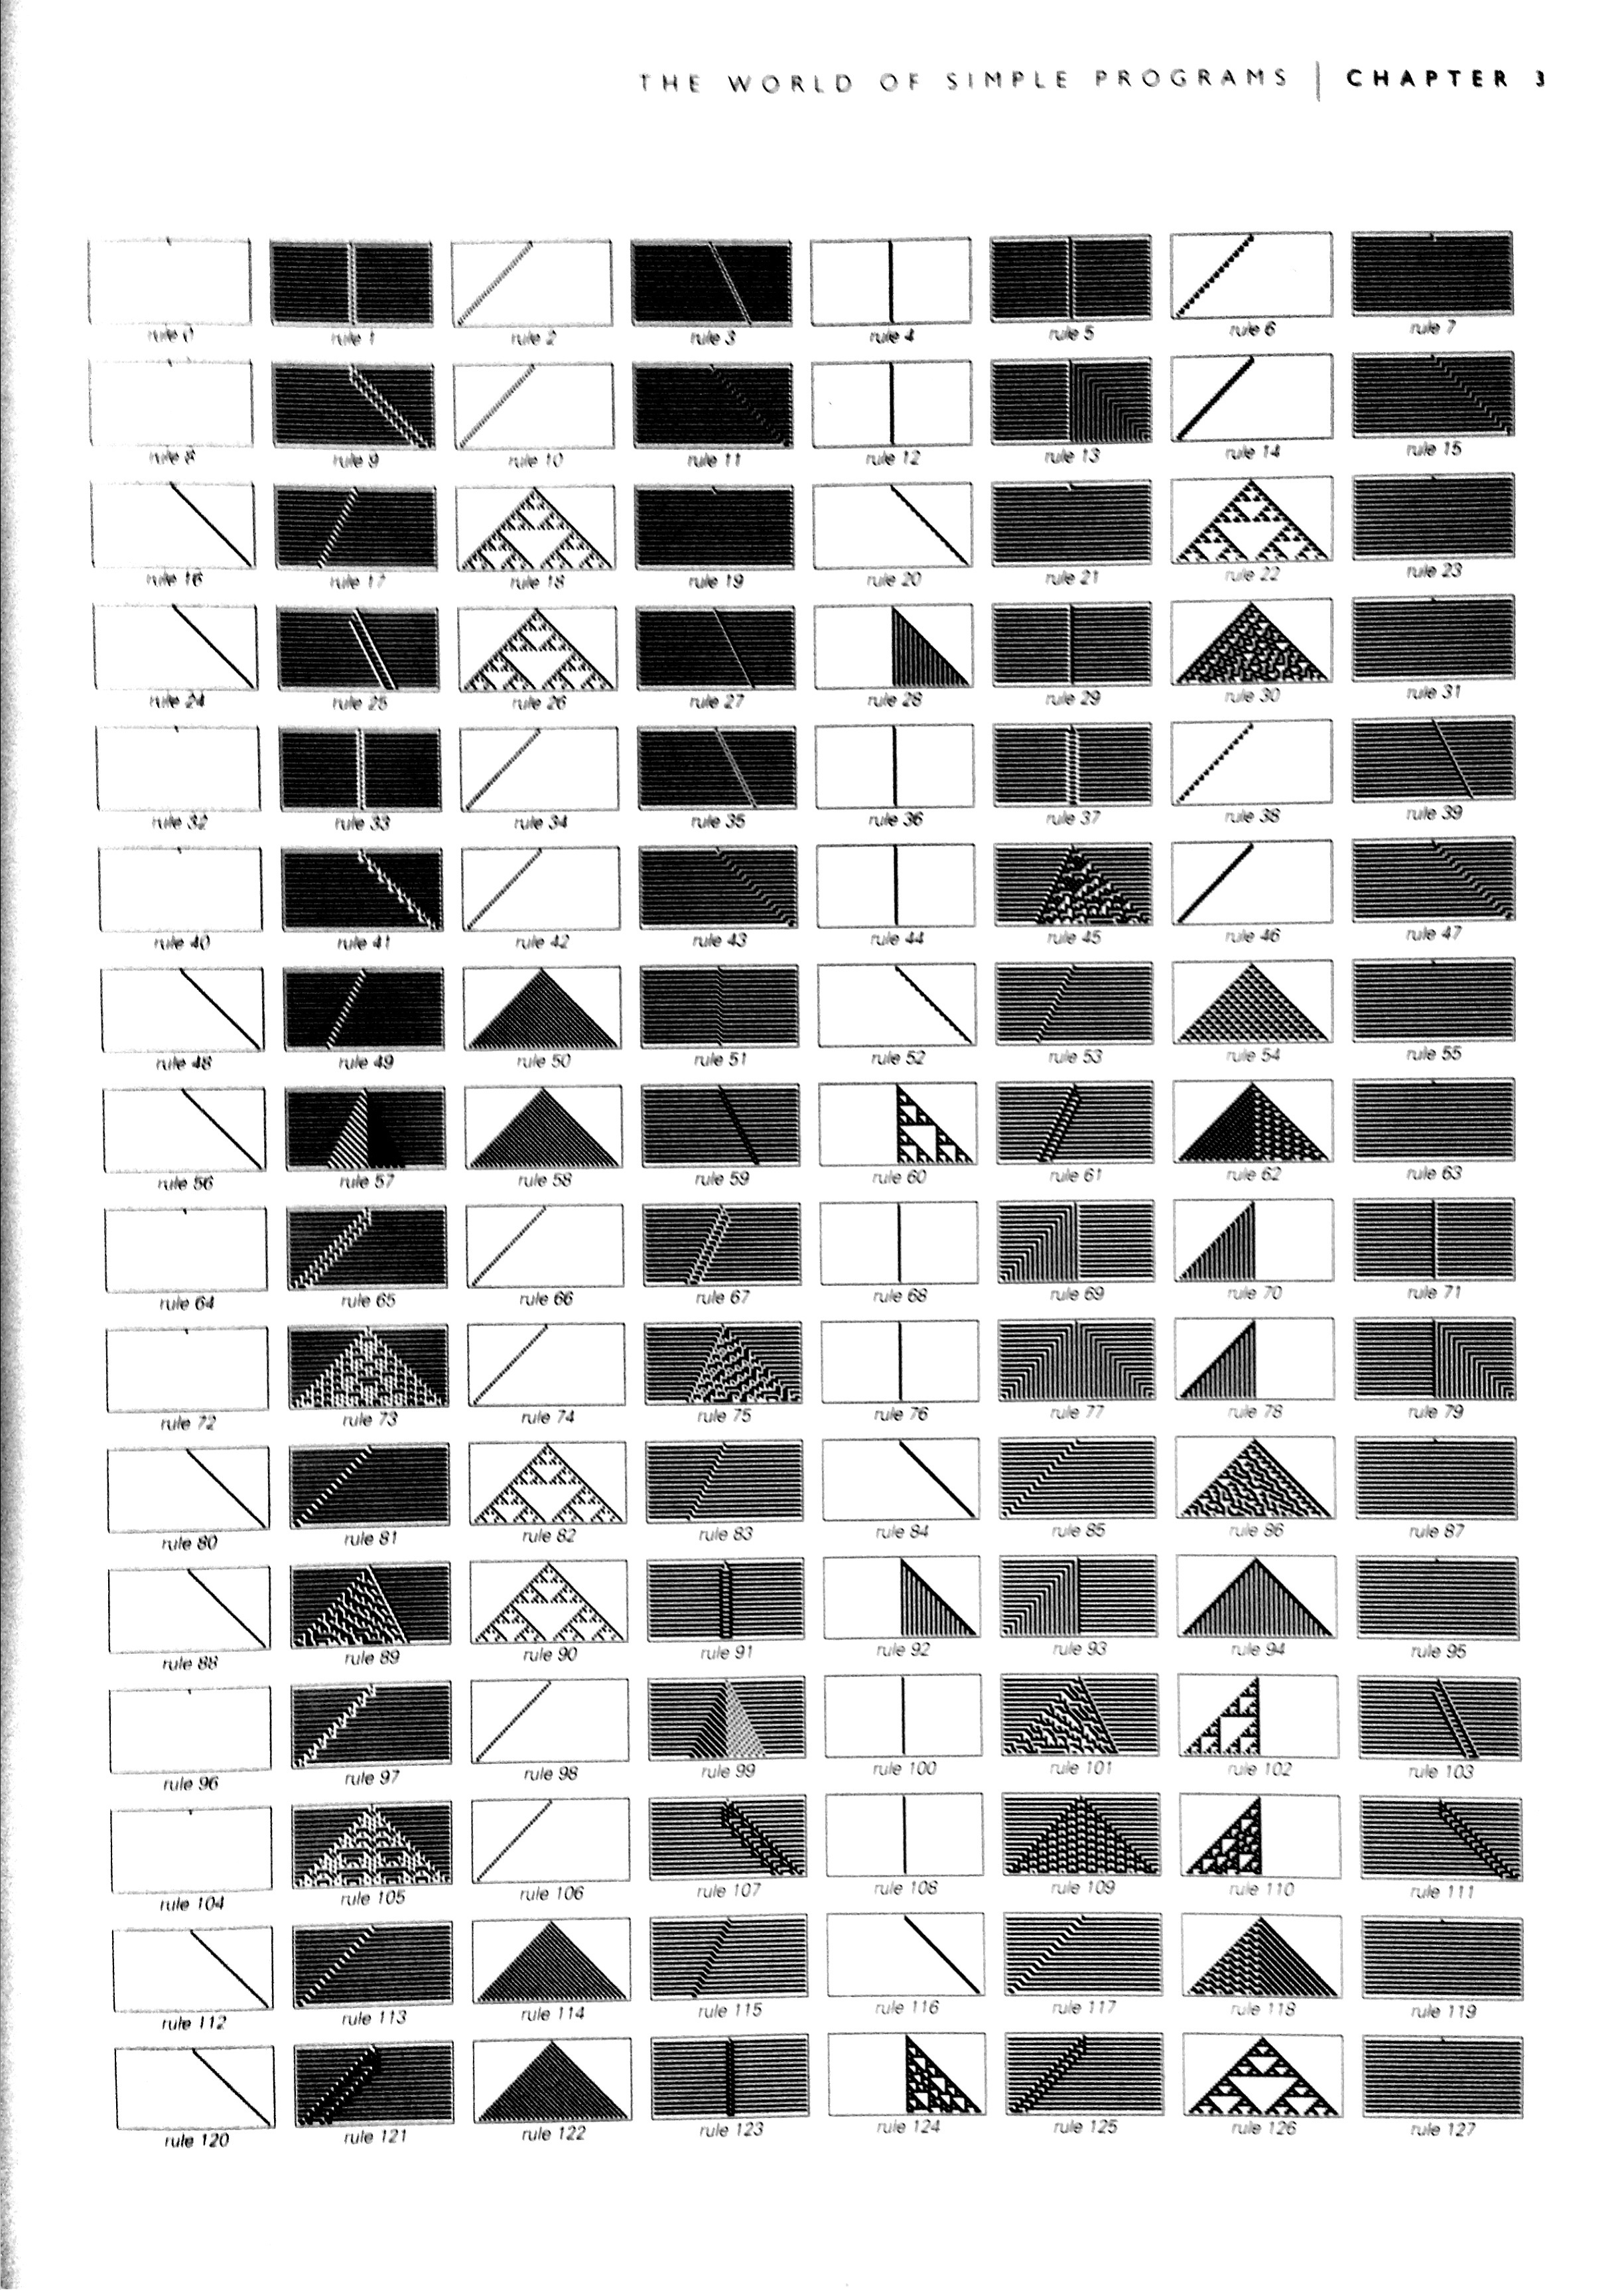
\includegraphics[width = 100]{lots}
\end{figure}

}

\section{Sandpile Model}
\frame
{
  \frametitle{Background}

  \begin{itemize}
  \item<1-> Imagine the dynamics of sandpile
  \item<2-> Drop one grain of sand in at a time
  \item<3-> Eventually the pile grows, until it reaches a point where the cells tumble
  \item<4-> Exhibits self-organized criticality
  	\begin{itemize}
	\item A critical state develops automatically
	\end{itemize}
  \item<5-> Back, Tang and Weisenfeld ($1977 \& 1978$)
  \end{itemize}
}

\subsection{Model}
\frame
{
  \frametitle{Conditions}

  \begin{itemize}
  \item Consider a 100x100 square lattice
  \item 4 neighbors (von Neumann)
  \item Free boundary
  \item Continuous time variable
   \end{itemize}
}


\frame
{
 \frametitle{Transition Rules}
 \begin{itemize}
  \item<1-> Each cell i holds a value $z_{i}$, if $z_{i}  > z_{c}$, the cell will 'tumble'
  \item<2-> When a cell tumbles, it affects its neighbors $z_{j}$'s values
  \begin{itemize}
  \item $z_{i} - 4$
  \item $z_{j} + 1$
  \end{itemize}
  \item <3->Stable $z_{i}$ values are  $0,1,2,3$ where $z_{c} = 3$
  \item <4->Two initial states considered: homogeneous or heterogeneous
\end{itemize}

}


\subsection{Results}
\frame
{
  \frametitle{Avalanches}

  \begin{itemize}
  \item A cell is considered apart of an avalanche if it tumbles at least once
  \item Size is the number of cells included in the avalanche
  \item Duration is the number of times the computer iterates through the entire lattice   
  \item See code (handout)
  \end{itemize}
}

\frame
{
  \frametitle{Homogeneous Initial State}

   \begin{figure}
   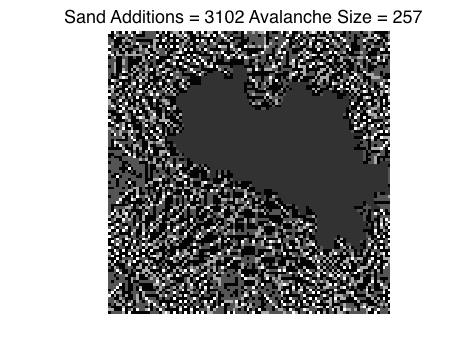
\includegraphics[width = 250]{avalanchehomo}
   \end{figure}

}

\frame
{
  \frametitle{Heterogeneous Initial State}

   \begin{figure}
   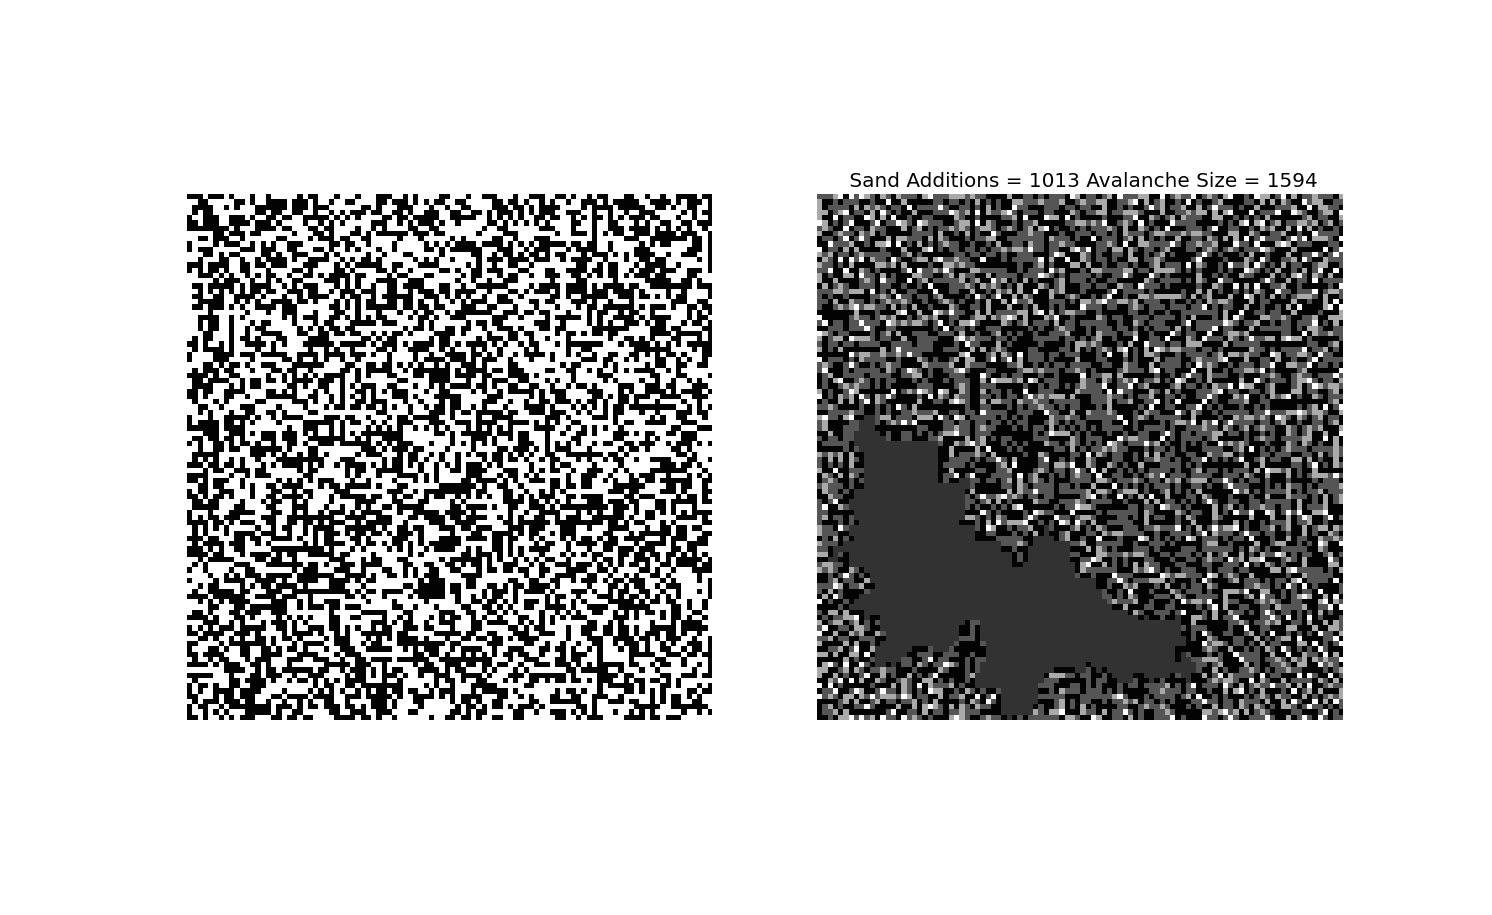
\includegraphics[width = 300]{avalanchehetero}
   \end{figure}

}

\frame
{
  \frametitle{Heterogeneous Initial State}

   \begin{figure}
   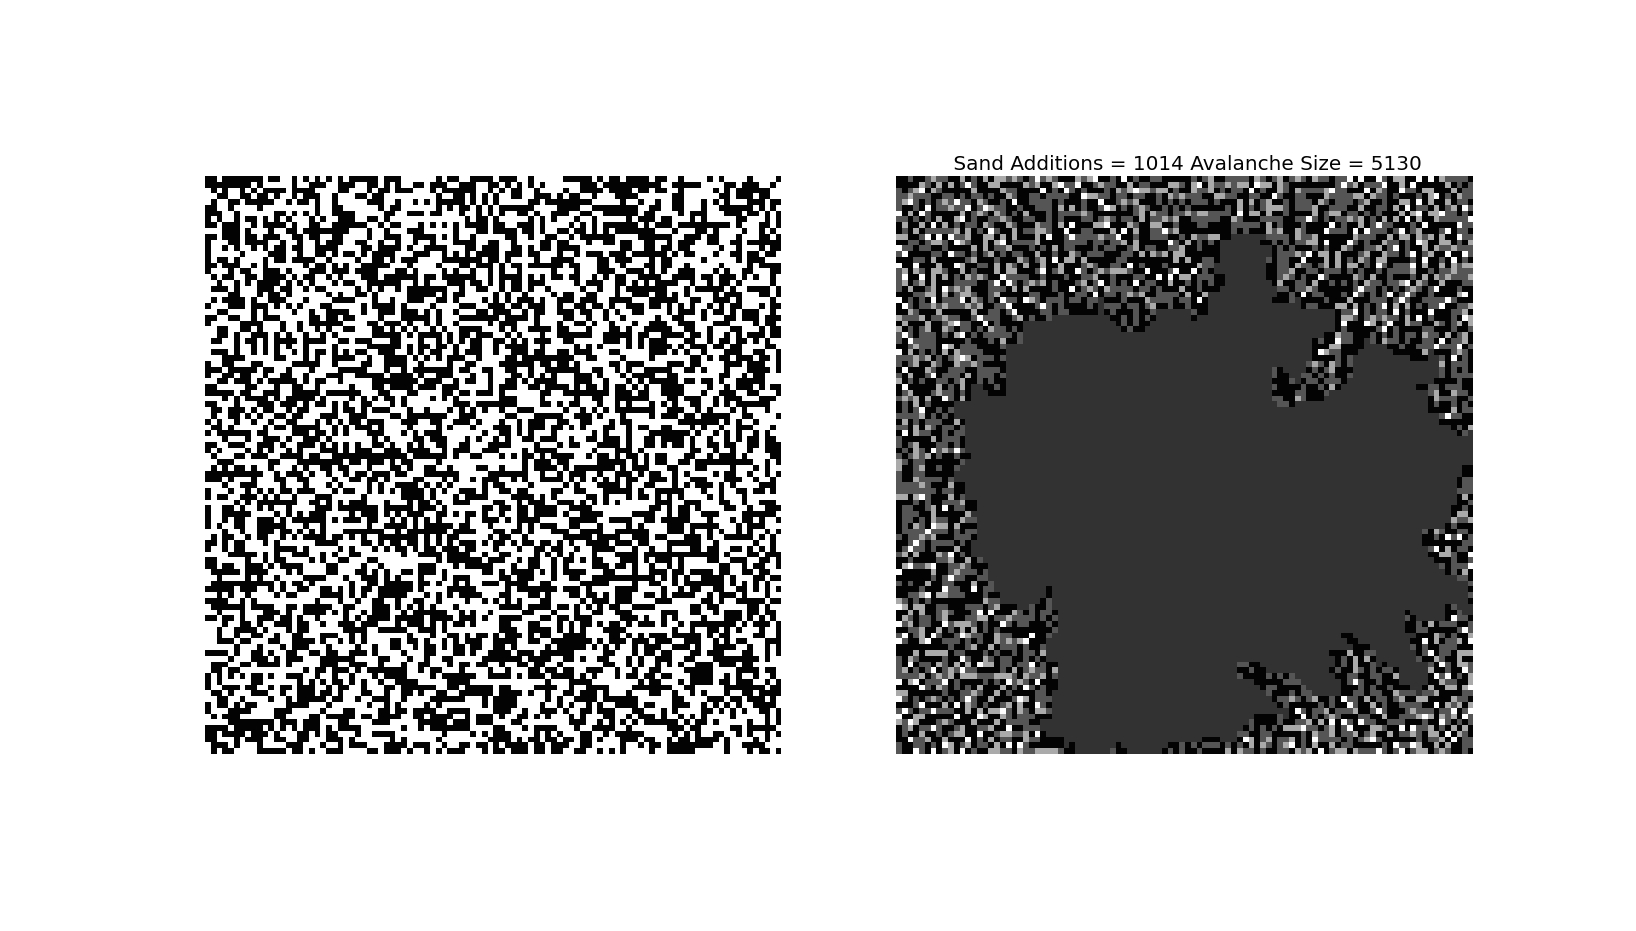
\includegraphics[width = 300]{bigavalanchehetero}
   \end{figure}

}


\subsection{Properties}
\frame
{
  \frametitle{Distribution of Avalanche Sizes}

  \begin{itemize}
  \item<1-> Avalanche frequency depends on their size by a power law
  \item<2-> $N(s) \sim s^{-\tau}$ where $\tau \approx 1.0$

  \end{itemize}
	
   \begin{figure}
   \includegraphics<3->[width = 200]{46a}
   \end{figure}
}

\frame
{
  \frametitle{Avalanche Duration Versus Size}

  \begin{itemize}
  \item<1-> $T(s) \sim s^{a}$ where $a \approx 0.65$

  \end{itemize}
	
   \begin{figure}
   \includegraphics<2->[width = 200]{46b}
   \end{figure}
}

\frame
{
  \frametitle{Frequency of Avalanche Duration}

  \begin{itemize}
  \item<1-> $N(t) \sim t^{-b}$  where $b \approx 1.1$

  \end{itemize}
	
   \begin{figure}
   \includegraphics<2->[width = 200]{46c}
   \end{figure}
}


\subsection{Snapshots}
\frame
{
  \frametitle{Relaxation of a System}

  \begin{itemize}
  \item<1-> Consider an avalanche's relaxation period, and see patterns it produces
  \end{itemize}
  
   \begin{figure}
   \includegraphics<2->[width = 250]{relaxation}
   \end{figure}
}

\frame
{
  \frametitle{My Snapshots}
    
   \begin{figure}
   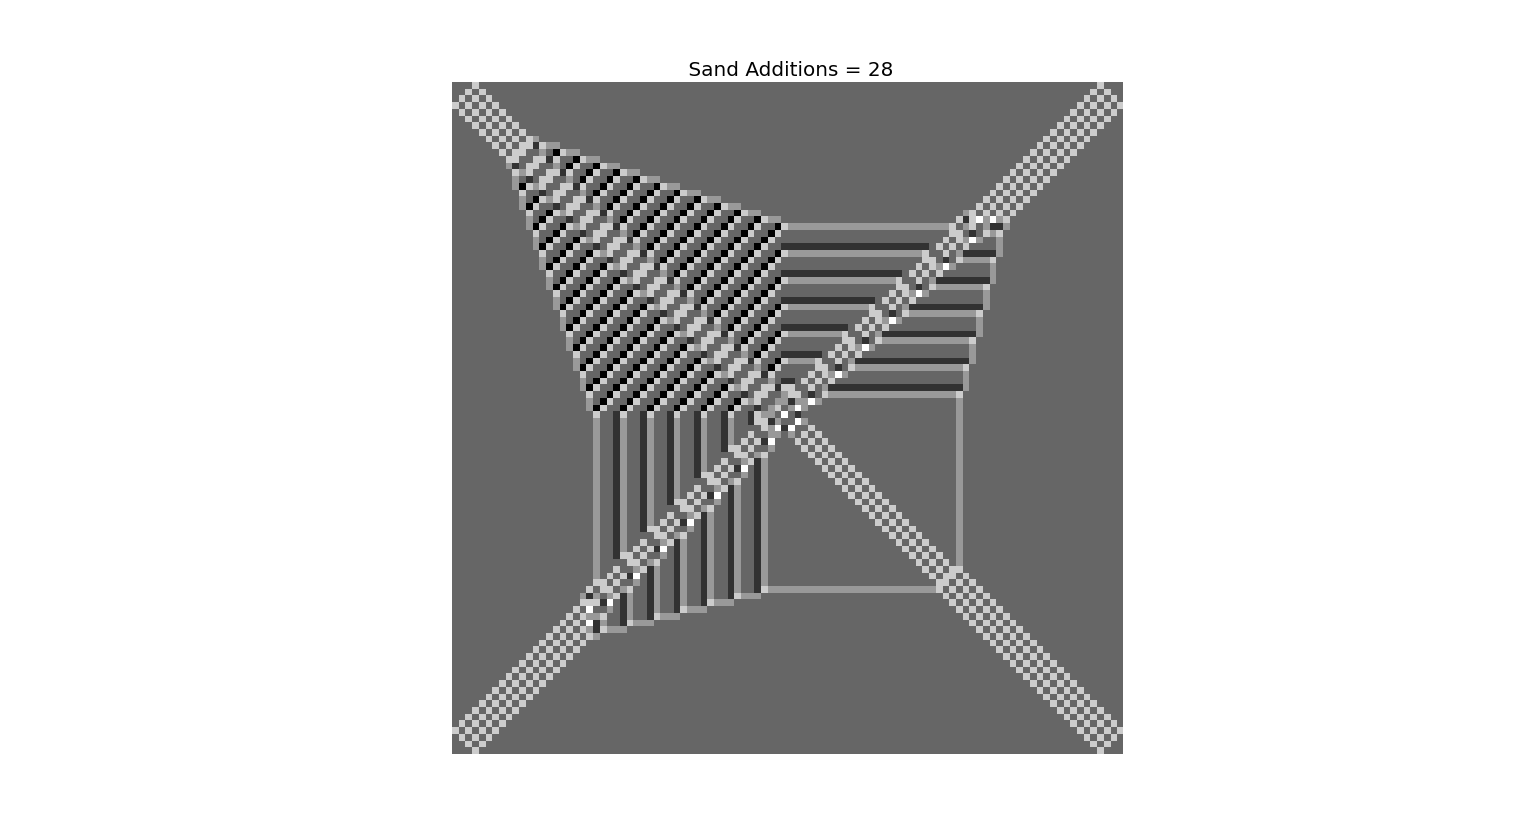
\includegraphics[width = 300]{centerhomo}
   \end{figure}
}

\frame
{
  \frametitle{My Snapshots}
    
   \begin{figure}
   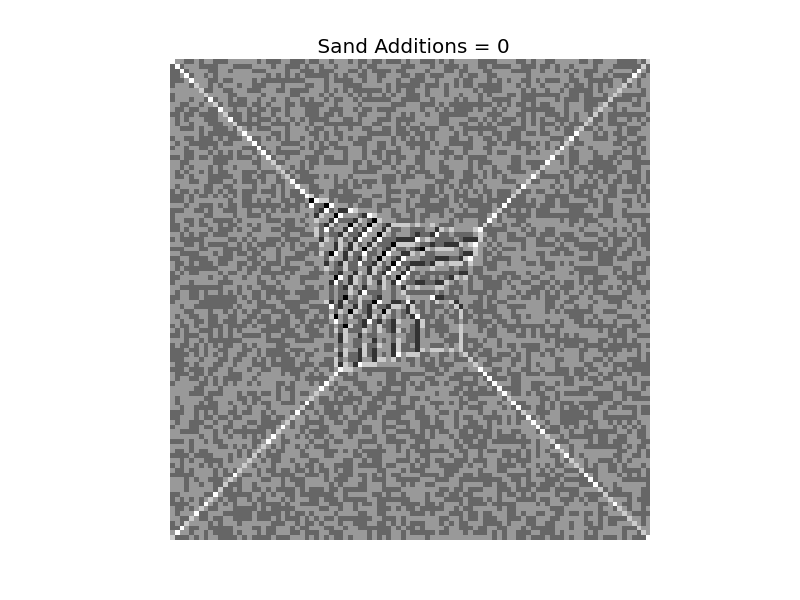
\includegraphics[width = 250]{center23}
   \end{figure}
}

\frame
{
  \frametitle{My Snapshots}
    
   \begin{figure}
   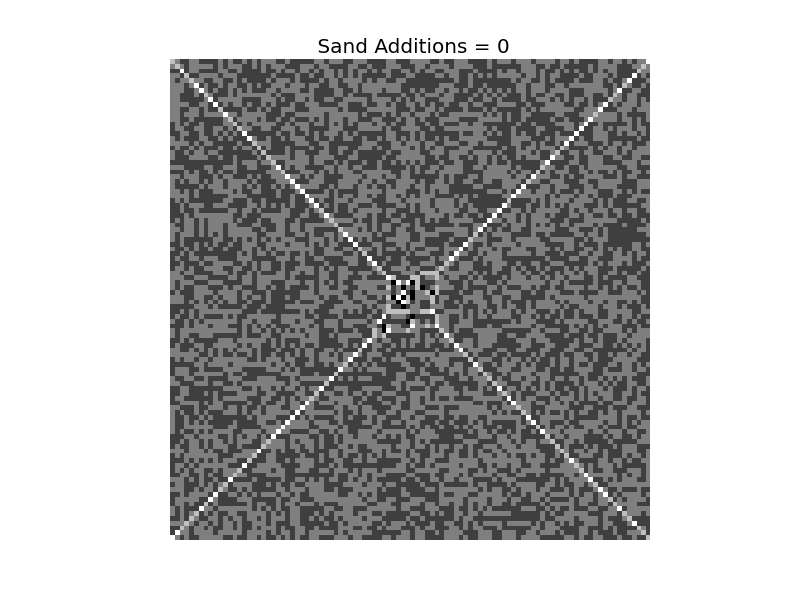
\includegraphics[width = 250]{blackcenter23}
   \end{figure}
}



\section{Conclusion}
\frame
{
  \frametitle{Future Questions}

  \begin{itemize}
  \item Vary boundary conditions
  \item Introduce damage
  \item 3D avalanche
  \end{itemize}
 
 }


\section{Cited}
\frame
{
  \frametitle{Works Cited}

  \begin{itemize}
  \item Computational Physics (2nd addition) by Nicholas Giordano and Hisao Nakanishi
  \item Bio-Inspired Artificial Intelligence by Dario Floreano and Claudio Mattiussi
  \end{itemize}
}


\end{document}